\section{Prediction Experiments}
\label{sec:exp_pred}

\begin{figure}
    \centering
    \begin{subfigure}[c]{0.99\linewidth}
        \centering
        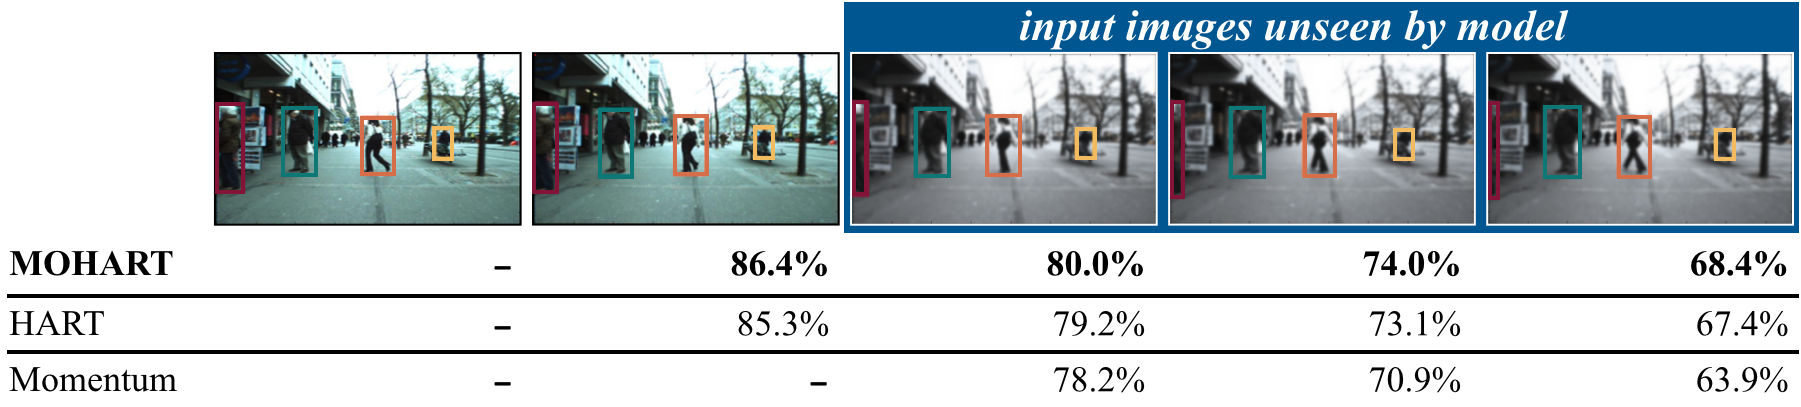
\includegraphics[width=\linewidth]{figures/MOHART/prediction_motc2.png}
        \vspace{-6mm}
        \caption{Prediction results on the MOTChallenge dataset \cite{Mot16}.}
        \label{fig:MOTC_imgs}
    \end{subfigure}
    \vspace{2mm}
    \begin{subfigure}[c]{0.99\linewidth}
        \centering
        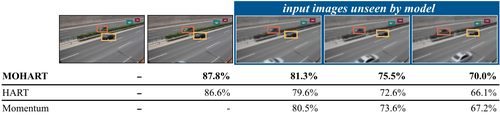
\includegraphics[width=\linewidth]{figures/MOHART/prediction_detrac2.png}
        \vspace{-6mm}
        \caption{Prediction results on the UA-DETRAC dataset (crowded scenes only) \cite{Wen15}.}
        \label{fig:Detrac_quant}
    \vspace{-5mm}
    \end{subfigure}
\caption{Peeking into the future. Only the first two frames are shown to the tracking algorithm followed by three black frames. \textsc{mohart} learns to fall back on its internal motion model when no observation (i.e. only a black frame) is available. The reported IoU scores show the performance for the respective frames 0, 1, 2, and 3 time steps into the future.
\label{fig:prediction}
}
\end{figure}

In the results from the \textit{prediction} experiments (see \Cref{fig:prediction}) \textsc{mohart} consistently outperforms \textsc{hart}. On both datasets, the model outperforms a baseline which uses momentum to linearly extrapolate the bounding boxes from the first two frames. This shows that even from just two frames, the model learns to capture motion models which are more complex than what could be observed from just the bounding boxes (i.e. momentum), suggesting that it uses visual information (\textsc{hart} \& \textsc{mohart}) as well as relational reasoning (\textsc{mohart}). The strong performance gain of \textsc{mohart} compared to \textsc{hart} on the UA-DETRAC dataset, despite the small differences for tracking on this dataset, can be explained as follows: this dataset features little interactions but strong correlations in motion. Hence when only having access to the first two frames, \textsc{mohart} profits from estimating the velocities of multiple cars simultaneously.